%%%%%%%%%%%
%% Home work template for Graduate School
%% Author : Thamme Gowda N.
%% Originally from  https://github.com/thammegowda/hw-tex-templ
%%%%%%%%%%%%%%

\documentclass[a4paper,doc,notimes]{article}
\usepackage[a4paper,margin=1in,footskip=0.25in]{geometry}
%%\documentclass[tikz]{standalone}
\usepackage{tikz}
%Required by APA6 package
\usepackage[normalem]{ulem}
\usepackage[english]{babel}
\usepackage[utf8x]{inputenc}
\usepackage{amsmath}
\usepackage{amssymb}
\usepackage{amsfonts}
\usepackage{graphicx}
\usepackage{adjustbox}

%Oft-used, oft-abused
\usepackage{afterpage}
\usepackage{booktabs}
\usepackage{caption}
\usepackage{censor}
\usepackage{color}
\usepackage{csquotes}
\usepackage{enumitem}
\usepackage{float}
\usepackage{hyperref}
\usepackage{lmodern}
%\usepackage{media9}
\usepackage{multirow}
\usepackage{outlines}
\usepackage{pdfpages}
\usepackage{placeins}
\usepackage{soul}
\usepackage{tabularx}
\usepackage[colorinlistoftodos]{todonotes}
\usepackage{xcolor}
\usepackage{mathtools}
\graphicspath{ {images/}}

\usepackage{sectsty}
\sectionfont{\fontsize{14}{12}\selectfont}

\setenumerate[1]{label=\Roman*.}
\setenumerate[2]{label=\Alph*.}
\setenumerate[3]{label=\roman*.}
\setenumerate[4]{label=\alph*.}

% break page where ever is required
\allowdisplaybreaks
\renewcommand{\thesubsection}{\thesection.\alph{subsection}}
\usepackage{titling}
\setlength{\droptitle}{-9em}
\newcommand\numberthis{\addtocounter{equation}{1}\tag{\theequation}}
\usepackage{listings}

\title{\noindent  \textbf{ USC CSCI 567 HOMEWORK 5 SOLUTIONS} }
\author{\textbf{ThammeGowda Narayanaswamy} \\
EMail: tnarayan@usc.edu  USCID: 2074-6694-39}

\date{} %% NO date

\begin{document}
\maketitle


\section{Clustering}
\subsection{}
Given that 
\begin{equation}\label{e:sse}
	D = \sum_{n=1}^{N} \sum_{k=1}^{K} r_{nk} \parallel x_n - \mu_k \parallel^2_2 = \sum_{n=1}^{N} \sum_{k=1}^{K} r_{nk} (x_n - \mu_k)^2
\end{equation}
By using the fact: the $argmin_{\mu_k}$ for \ref{e:sse} is when its first order partial derivative is zero.

\begin{align*}
  \frac{\partial}{\partial \mu_k} \sum_{n=1}^{N} \sum_{k'=1}^{K} r_{nk'} (x_n - \mu_{k'})^2 =& 0 & \\
   \sum_{n=1}^{N} r_{nk} x_n - \mu_k \sum_{n=1}^{N} r_{nk}  =& 0 & \\ 
   \implies \mu_k^* =& \frac{1}{\sum_{n=1}^{N} r_{nk}} \sum_{n=1}^{N} r_{nk} x_n \numberthis \label{e:mean}
\end{align*}
The equation \ref{e:mean} implies that the $\mu_k^*$ is the mean of the data points in the cluster $k$.

\subsection{}
Given that 
\begin{equation}\label{e:l1norm}
	D = \sum_{n=1}^{N} \sum_{k=1}^{K} r_{nk} | x_n - \mu_k |_1 = \sum_{n=1}^{N} \sum_{k=1}^{K} r_{nk} sign(x_n - \mu_k) (x_n - \mu_k)
\end{equation}
By using the fact: the $argmin_{\mu_k}$ for \ref{e:l1norm} is when its first order partial derivative is zero.
\begin{align*}
 \frac{\partial}{\partial \mu_k}\sum_{n=1}^{N} \sum_{k=1}^{K} r_{nk} sign(x_n - \mu_k) (x_n - \mu_k) =& 0 & \\
 \sum_{n=1}^{N} \sum_{k=1}^{K} - r_{nk} sign(x_n - \mu_k) =& 0 & \numberthis \label{e:median}
\end{align*}
Now if we interpret the meaning of \ref{e:median}, we get the following:
\begin{itemize}
	
	\item $sign(x_n - \mu_k)$ is $+1$ when $x_n > \mu_k$ and $-1$ when $x_n < \mu_k$
	\item Equation \ref{e:median} is lower when there are equal number of $x_n > \mu_k$ and $x_n < \mu_k$
	\item $\implies$ that $\mu_k$ is the median of $x$ . This argument holds for both the cases of even and odd number of points in the dataset.
\end{itemize}

\subsection{}

Given
\begin{equation}
	\tilde{D} = \sum_{n=1}^{N} \sum_{k=1}^{K} r_{nk} \parallel\phi(x_n) - \tilde{\mu_k} \parallel_2^2 \\
\end{equation}
\subsubsection{}
\begin{align*}
\implies \tilde{D} = & \sum_{n=1}^{N} \sum_{k=1}^{K} r_{nk} [\phi(x_n) - \tilde{\mu_k}]^T [\phi(x_n) - \tilde{\mu_k}] \\
 =& \sum_{n=1}^{N} \sum_{k=1}^{K} r_{nk} [\phi(x_n)^T\phi(x_n) + \tilde{\mu_k}^2 - 2 \phi(x_n) \tilde{\mu_k} ] \\
  & \text{By subsituting } k(x_1, x_2) = \phi(x_1)^T\phi(x_2) \\
 =& \sum_{n=1}^{N} \sum_{k=1}^{K} r_{nk} [k(x_n, x_n) + \tilde{\mu_k}^2 - 2 \phi(x_n) \tilde{\mu_k} ] \numberthis \label{e:D1} \\
\end{align*}
Using \ref{e:mean} to simplify the middle term of \ref{e:D1}, we have 
\begin{align*}
	\tilde{\mu_k} =& \frac{1}{\sum_{i=1}^{N} r_{ik}} \sum_{i=1}^{N} r_{ik} \phi(x_i) 
				 = \frac{1}{N_k} \sum_{i=1}^{N} r_{ik} \phi(x_i) \numberthis \label{e:mean2}& \space  \because N_k = \sum_{i=1}^{N} r_{ik} \\	
 =& \frac{1}{N_k^2} \sum_{i=1}^{N} r_{ik} \sum_{j=1}^{N} r_{jk} \phi(x_i)^T\phi(x_j) \\ 
 & \text{By subsituting } k(x_1, x_2) = \phi(x_1)^T\phi(x_2) \\
 \tilde{\mu_k}^2 =& \frac{1}{N_k^2} \sum_{i=1}^{N} r_{ik} \sum_{j=1}^{N} r_{jk} k(x_i, x_j) \numberthis \label{e:D2}
\end{align*}
Simplifying the last term of \ref{e:D1},
\begin{align*}
 \phi(x_n) \tilde{\mu_k} & = \phi(x_n) \frac{1}{N_k} \sum_{i=1}^{N} r_{ik} \phi(x_i) = \frac{1}{N_k} \sum_{i=1}^{N} r_{ik} \phi(x_n)^T \phi(x_i) \\
 & \text{By subsituting } k(x_1, x_2) = \phi(x_1)^T\phi(x_2) \\
\phi(x_n) \tilde{\mu_k} &= \frac{1}{N_k} \sum_{i=1}^{N} r_{ik} \times k(x_n, x_i) \numberthis \label{e:D3}
\end{align*}
Substituting \ref{e:D2} and \ref{e:D3} in \ref{e:D1}, we have:
\begin{align*}
\tilde{D} =& \sum_{n=1}^{N} \sum_{k=1}^{K} r_{nk} \bigg[k(x_n, x_n) +  \frac{1}{N_k^2} \sum_{i=1}^{N} r_{ik} \sum_{j=1}^{N} r_{jk} \times k(x_i, x_j) - 2 \frac{1}{N_k} \sum_{i=1}^{N} r_{ik} \times k(x_n, x_i) \bigg] \numberthis \label{e:D4} \\
& \text{where } N_k = \sum_{i=1}^{N} r_{ik}
\end{align*}
We note that, the $L_2$ norm difference between mean of cluster to $x_n$ is given by (used later)
\begin{equation} \label{e:D5}
 \parallel\phi(x_n) - \tilde{\mu_k} \parallel_2^2 = k(x_n, x_n) +  \frac{1}{N_k^2} \sum_{i=1}^{N} r_{ik} \sum_{j=1}^{N} r_{jk} \times k(x_i, x_j) - 2 \frac{1}{N_k} \sum_{i=1}^{N} r_{ik} \times k(x_n, x_i)
\end{equation}

%%%%%%%%%%%%%%%%
\subsubsection{}
To assign a data point $x_n$ to a cluster, we first compute the value of \ref{e:D5} for all the clusters $k \in 1, 2, K$. Then assign it to a the cluster with minimum distance. i.e
\begin{equation}\label{e:asgn}
	A(x_n) = argmin_k \parallel x_n - \mu_k \parallel^2_2 
\end{equation}
where $A(x_n)$ stores the cluster assignment of $x_n$

\subsubsection{Pseudo code}
\begin{lstlisting}[mathescape=true]
function kernel_k_means(k, X, K):
  Parameters:
    k : Number of clusters
    X : Array of data points
    K : Kernel Function
  Returns:
    $A(x_n)$: cluster assignments for all the points in X

  Step 1: Initialize centroids of k clusters to
         some random points in the dataset
      for i in range(k):
        $\mu_k \leftarrow random$

  Step 2: Compute the assignment of points
      for n in range(N):
        $A(x_n) \leftarrow argmin_k \parallel x_n - \mu_k \parallel^2_2 $ # Use equation $\ref{e:D5}$ to compute

  Step 3: Recompute the mean/centroid of cluster
      for i in range(k):
        $\mu_k \leftarrow$ Use equation $\ref{e:mean2}$ to compute the mean
  
  Step 4: Check for termination
      if the values of $\mu_k$ does not change:
        return $A(x_n)$ for all $x_n$
      else:
        go to Step 2
\end{lstlisting}
\section{Gaussian Mixture Model}
\subsection{}

\begin{align*}
L = & P(x_1|\alpha) = \alpha f(x_1|\theta_1) + (1 - \alpha) f(x_1|\theta_2) = \alpha N(0, 1) + (1 - \alpha) N(0, 0.5)  & \\
L = & \frac{\alpha}{\sqrt{2 \pi}} e^{-\frac{x_1^2}{2}} + \frac{1 - \alpha}{\sqrt{\pi}} e^{-x_1^2} & \\
= & \big[\frac{1}{\sqrt{2 \pi}} e^{-\frac{x_1^2}{2}} - \frac{1}{\sqrt{\pi}} e^{-x_1^2} \big] \times \alpha + \frac{1}{\sqrt{\pi}} e^{-x_1^2} \numberthis \label{e:2a1} &  \\
\end{align*}

Note that the above equation is of form $m \alpha + c$ which is a linear in $\alpha$ \\ where $m = \frac{1}{\sqrt{2 \pi}} e^{-\frac{x_1^2}{2}} - \frac{1}{\sqrt{\pi}} e^{-x_1^2}$ and $c = \frac{1}{\sqrt{\pi}} e^{-x_1^2}$ \\
The maximum likelihood estimation of $\alpha$ as follows.
\begin{enumerate}
	\item When $m$ is positive, that is when $\frac{1}{\sqrt{2 \pi}} e^{-\frac{x_1^2}{2}} > \frac{1}{\sqrt{\pi}} e^{-x_1^2}$, we chose maximum value i.e. $\alpha=1$
	\item When $m$ is negative, that is when $\frac{1}{\sqrt{2 \pi}} e^{-\frac{x_1^2}{2}} < \frac{1}{\sqrt{\pi}} e^{-x_1^2}$, we chose minimum value i.e $\alpha=0$
\end{enumerate}

Alternatively we can also use an iterative algorithm such as Expectation Maximization algorithm to compute the above.

\section{EM algorithm}

Given Zero-inflated Poisson Distribution:

\begin{equation}\label{e:observed}
p(x_i) = \begin{cases}
\pi + (1-\pi) e^{-\lambda} & \text{if } x_i = 0\\
(1-\pi) \frac{\lambda^{x_i} e^{-\lambda}}{x_i!} &  \text{if } x_i > 0
\end{cases}
\end{equation}
\subsection{}

For every observation $x_i=0$, let us introduce an hidden indicator variable $z_i$ to indicate whether or not the observation from Zero inflation or Poisson process. i.e. 

\begin{equation}\label{e:hidden}
z_i = \begin{cases}
1,& \text{if } x_i \text{from zero inflation}\\
0,&  \text{if } x_i \text{from poisson process} 
\end{cases}
\end{equation}
Using \ref{e:observed} and \ref{e:hidden}, we can rewrite PDF $\forall x_i \ge 0 $ as the following:

\begin{equation}\label{e:combines}
p(x_i) = \begin{cases}
\pi^{z_i} \times ((1-\pi) e^{-\lambda})^{1-z_i} & \text{if } x_i = 0, z_i \in{0,1}\\
(1-\pi) \frac{\lambda^{x_i} e^{-\lambda}}{x_i!} &  \text{if } x_i > 0
\end{cases}
\end{equation}


The likelihood of parameters $\lambda$ and $\pi$ in \ref{e:combined} based on $N$ observations in dataset $D$ is given by
\begin{align*}
L = & \prod_{i=1}^{N} p(x_i) = \prod_{i:x_i=0}^{N} p(x_i) \times \prod_{i:x_i \ge 0}^{N} p(x_i) \\
L = &  \prod_{i:x_i=0}^{N} \pi^{z_i} \times ((1-\pi) e^{-\lambda})^{1-z_i} \times \prod_{i:x_i \ge 0}^{N} (1-\pi) \frac{\lambda^{x_i} e^{-\lambda}}{x_i!} \numberthis \\
& \text{The log likelihood is} \\
log L = & log \bigg[ \prod_{i:x_i=0}^{N} \pi^{z_i} \times ((1-\pi) e^{-\lambda})^{1-z_i} \times \prod_{i:x_i \ge 0}^{N} (1-\pi) \frac{\lambda^{x_i} e^{-\lambda}}{x_i!} \bigg] \\
= & \sum_{i:x_i=0}^{N} \big[z_i \log \pi +  (1 - z_i)[\log (1- \pi) -\lambda]\big] 
  + \sum_{i:x_i \ge 0}^{N} \big[\log(1- \pi) + x_i \log \lambda -\lambda - \log x_i! \big] \numberthis \label{e:loglike}
\end{align*}
\subsection{}
For the E-step, we need to find probability of hidden variables. This is done by following
\begin{align*}
	P(z_i=1|x_i, \lambda, \pi) & = \frac{P(x_i=0|z_i=1, \lambda, \pi) \times P(z_i=1)}{P(x_i=0)} = \frac{\pi}{\pi + (1-\pi)e^{-\lambda}} = \gamma_{i1} \\
	P(z_i=0|x_i=0, \lambda, \pi) & = \frac{P(x_i=0|z_i=0, \lambda, \pi) \times P(z_i=0)}{P(x_i=0)} = \frac{(1-\lambda)e^{-\lambda}}{\pi + (1-\pi)e^{-\lambda}} = \gamma_{i0}
\end{align*}

For the M-step we need to find the better estimate of parameters $\pi$ and $\lambda$.

We define a function $Q(\theta^t, \theta^{t-1})$ 
\begin{align*}
Q(\theta^t, \theta^{t-1}) &= E_{P(Z|X, \lambda^{t-1}, \pi^{t-1})}[log(P(X,Z|\lambda,\pi))] \\
  &= \sum_{i:x_i=0}^{N} \big[E[z_i] \log \pi +  E[1 - z_i][\log (1- \pi) -\lambda]\big] 
  + \sum_{i:x_i \ge 0}^{N} \big[\log(1- \pi) + x_i \log \lambda -\lambda - \log x_i! \big] \\
  &= \sum_{i:x_i=0}^{N} \big[\gamma_{i1} \log \pi +  \gamma_{i0}[\log (1- \pi) -\lambda]\big] 
  + \sum_{i:x_i \ge 0}^{N} \big[\log(1- \pi) + x_i \log \lambda -\lambda - \log x_i! \big] \numberthis \label{e:Q}
\end{align*}
The update rule can be obtained by finding the derivative of \ref{e:Q} w.r.t $\lambda$ and $\pi$.
\begin{align*}
	\frac{\partial Q}{\partial \lambda} & = \sum_{i:x_i=0}^{N} \gamma_{i0} + \sum_{i:x_i \ge 0}^{N} [\frac{x_i}{\lambda} -1 ] \numberthis \\
	\frac{\partial Q}{\partial \pi} &= \sum_{i:x_i=0}^{N} (\frac{\gamma_{i1}}{\pi} - \frac{\gamma_{i0}}{(1-\pi)}) + \sum_{i:x_i \ge 0}^{N} \frac{-1}{1-\pi}	 \\
	\implies & \lambda^{t+1} = \frac{\sum_{i=1}^{N}}{\sum_{i:x_i>0}^{N} 1 + \sum_{i:x_i=0}^{N} \gamma_{i0} }  \text { and }  \pi^{t+1} = \sum_{i:x_i=0}^{N} \frac{\gamma_{i1}}{N}  \\
\end{align*}
\section{Programming}
\stepcounter{subsection}
\subsection{K means}
\subsubsection \\
\includegraphics*[scale=0.5]{k_means.png}

\subsubsection{}
\begin{enumerate}
	\item The circles dataset is not linearly separable. K means doesn't have right objective function to optimize. 
\end{enumerate}

\subsection{Kernel K means}
\subsubsection{Kernel}

\begin{align*}
    & k(x_1, x_2) \leftarrow 1.0 - \frac{min(r1, r2)}{ max(r1, r2)} \\
    \text{where  } &  r_1 \leftarrow || x_1 - 0 ||_2  \\
    \text{ and } & r_2 \leftarrow || x_2 - 0 ||_2 \\
    & \text{ and $0$ is the center of the cicles, in this data set it is origin of coordinate system}
\end{align*}

\subsubsection{}
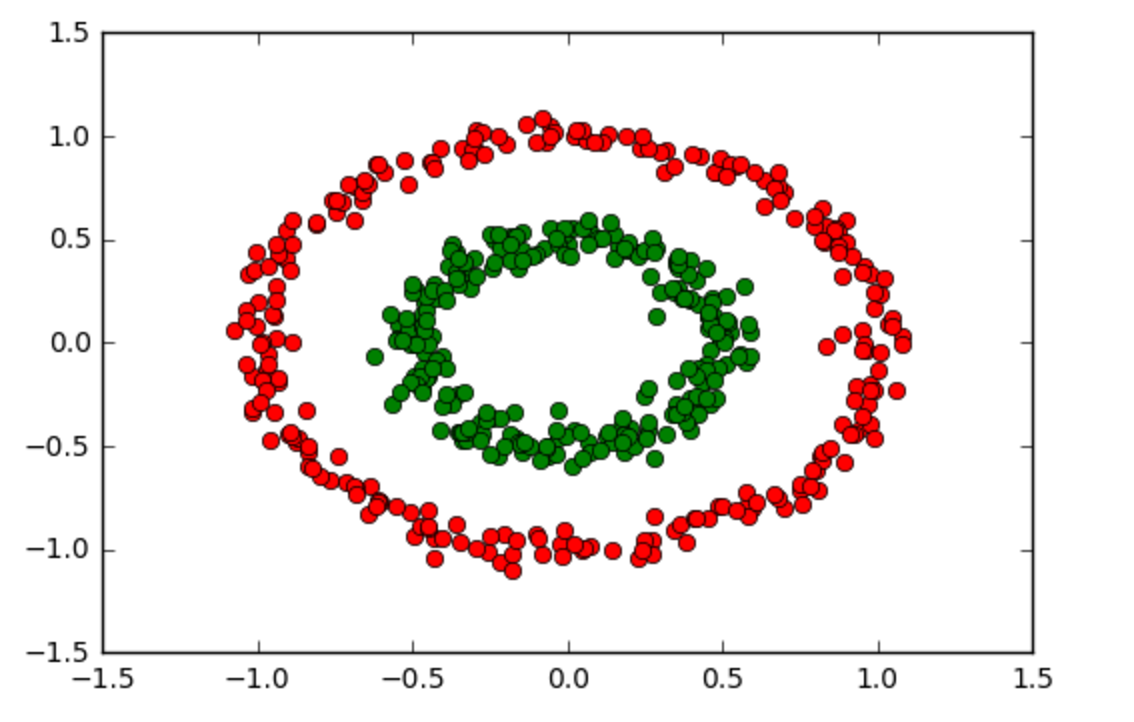
\includegraphics[scale=0.75]{images/kernel_kmeans.png}

\subsection{EM Algorithm}

\subsubsection{Log likelihood of EM}
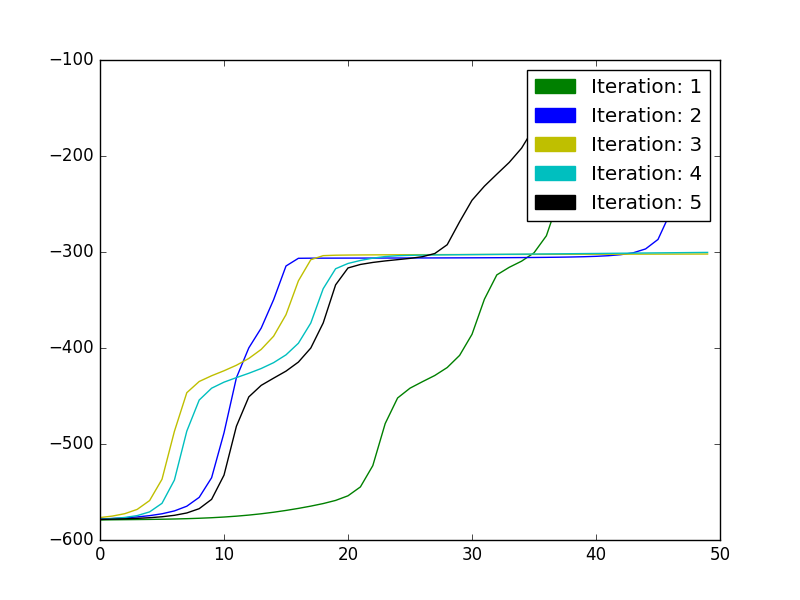
\includegraphics[scale=0.55]{loglikelihood.png}
\subsubsection{Best Cluster Assignment}

\textbf{Plot} \\
 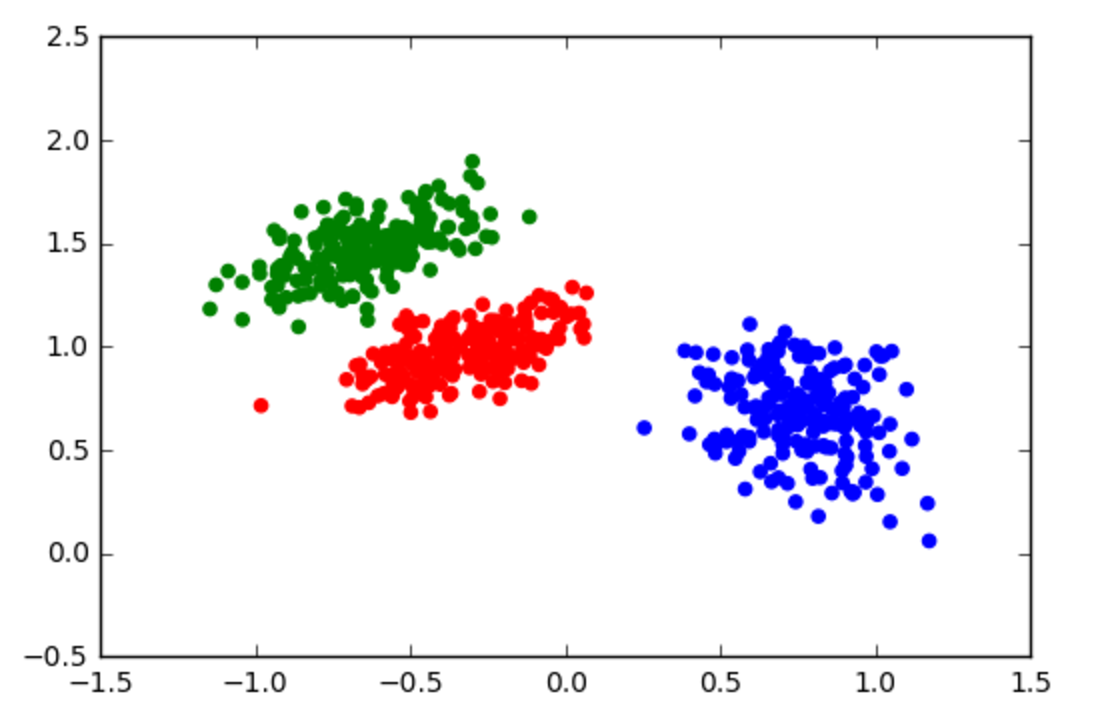
\includegraphics[scale=0.7]{em_clusters.png} \\

\textbf{Best Parameters}
\begin{verbatim}
Mean:
# 1
	[-0.3258436 ,  0.97128906]

# 2
	 [-0.63945162,  1.47450927]

# 3
	 [ 0.75896021,  0.67976991]

Covariance:
#1
		 [ 0.03603698,  0.01465574],
		 [ 0.01465574,  0.01628796]

#2
		  [ 0.03595904,  0.01548498],
		  [ 0.01548498,  0.01937919]

# 3
		 [ 0.02717059, -0.00840047],
		 [-0.00840047,  0.04044201]

\end{verbatim}

\end{document}